\chapter{动态规划}

\index{dynamic programming}

\key{动态规划}是一种兼具完整搜索的正确性与贪心算法效率的技术。当一个问题可以划分为相互重叠且能够独立求解的子问题时，就可以应用动态规划。

动态规划有两类用途：

\begin{itemize}
\item
\key{寻找最优解}：希望找到尽可能大或尽可能小的解。
\item
\key{统计解的数量}：希望计算所有可能解的总数。
\end{itemize}

我们先了解如何用动态规划寻找最优解，再用相同思想统计解的数量。

理解动态规划是每位竞赛程序员成长过程中的里程碑。它的基本思想虽然简单，难点却在于如何将其应用到不同问题。本章介绍一组经典问题，作为学习动态规划的良好起点。

\section{硬币问题}

首先讨论第 6 章已经见过的问题：给定硬币面值集合 $\texttt{coins}=\{c_1,c_2,\ldots,c_k\}$ 和目标金额 $n$，需要用尽可能少的硬币凑出 $n$。

第 6 章使用始终选择最大可用面值的贪心算法解决了该问题。对于欧元硬币等情形，这个算法是正确的；但在一般情形下，贪心算法不一定产生最优解。

现在用动态规划高效解决这个问题，使算法适用于任意硬币集合。动态规划算法以一个递归函数为基础，像暴力算法一样遍历凑出金额的所有可能方式。不过，动态规划使用\emph{记忆化}，每个子问题的答案只计算一次，因此十分高效。

\subsubsection{递归形式}

动态规划的思想是用递归形式描述问题，使原问题的解可以由更小子问题的解计算出来。对于硬币问题，一个自然的递归问题是：凑出金额 $x$ 最少需要多少枚硬币？

令 $\texttt{solve}(x)$ 表示凑出金额 $x$ 所需的最少硬币数。函数值取决于硬币的面值。例如，若 $\texttt{coins}=\{1,3,4\}$，函数开头的一些值如下：

\[
\begin{array}{lcl}
\texttt{solve}(0) & = & 0 \\
\texttt{solve}(1) & = & 1 \\
\texttt{solve}(2) & = & 2 \\
\texttt{solve}(3) & = & 1 \\
\texttt{solve}(4) & = & 1 \\
\texttt{solve}(5) & = & 2 \\
\texttt{solve}(6) & = & 2 \\
\texttt{solve}(7) & = & 2 \\
\texttt{solve}(8) & = & 2 \\
\texttt{solve}(9) & = & 3 \\
\texttt{solve}(10) & = & 3 \\
\end{array}
\]

例如，$\texttt{solve}(10)=3$，因为凑出 10 至少需要 3 枚硬币，最优解为 $3+3+4=10$。

$\texttt{solve}$ 的关键性质是，其值可以由较小的函数值递归计算出来。方法是关注为总金额选择的\emph{第一枚}硬币。在上述情形中，第一枚硬币可以是 1、3 或 4。如果首先选择面值 1，剩余任务就是用最少硬币凑出 9，这是原问题的子问题；面值 3 和 4 也同理。因此，可以用下列递推式计算最少硬币数：
\begin{equation*}
\begin{split}
\texttt{solve}(x) = \min( & \texttt{solve}(x-1)+1, \\
                           & \texttt{solve}(x-3)+1, \\
                           & \texttt{solve}(x-4)+1).
\end{split}
\end{equation*}
递归的基本情形为 $\texttt{solve}(0)=0$，因为凑出空金额不需要硬币。例如，
\[ \texttt{solve}(10) = \texttt{solve}(7)+1 = \texttt{solve}(4)+2 = \texttt{solve}(0)+3 = 3.\]

现在可以给出计算凑出金额 $x$ 所需最少硬币数的一般递归函数：
\begin{equation*}
    \texttt{solve}(x) = \begin{cases}
               \infty               & x < 0\\
               0               & x = 0\\
               \min_{c \in \texttt{coins}} \texttt{solve}(x-c)+1 & x > 0 \\
           \end{cases}
\end{equation*}

首先，若 $x<0$，函数值为 $\infty$，因为不可能凑出负金额。若 $x=0$，函数值为 0，因为凑出空金额不需要硬币。最后，若 $x>0$，变量 $c$ 遍历第一枚硬币的所有选择。

找到解决问题的递归函数后，就可以直接用 C++ 实现（常量 \texttt{INF} 表示无穷大）：

\begin{lstlisting}
int solve(int x) {
    if (x < 0) return INF;
    if (x == 0) return 0;
    int best = INF;
    for (auto c : coins) {
        best = min(best, solve(x-c)+1);
    }
    return best;
}
\end{lstlisting}

不过，这个函数仍然不够高效，因为凑出金额的方式可能有指数级多种。下面将使用一种称为记忆化的技术使函数高效运行。

\subsubsection{使用记忆化}

\index{memoization}

动态规划使用\key{记忆化}高效计算递归函数的值，也就是把计算出的函数值存入数组。对每个参数只递归计算一次函数值，此后可直接从数组中取出。

在这个问题中，使用数组
\begin{lstlisting}
bool ready[N];
int value[N];
\end{lstlisting}

其中 $\texttt{ready}[x]$ 表示 $\texttt{solve}(x)$ 是否已计算；若已计算，$\texttt{value}[x]$ 保存其值。常量 $N$ 的取值应确保所有需要的值都能放入数组。

现在可以高效地实现该函数：

\begin{lstlisting}
int solve(int x) {
    if (x < 0) return INF;
    if (x == 0) return 0;
    if (ready[x]) return value[x];
    int best = INF;
    for (auto c : coins) {
        best = min(best, solve(x-c)+1);
    }
    value[x] = best;
    ready[x] = true;
    return best;
}
\end{lstlisting}

函数仍像之前一样处理 $x<0$ 和 $x=0$ 两种基本情形。然后通过 $\texttt{ready}[x]$ 检查 $\texttt{solve}(x)$ 是否已存入 $\texttt{value}[x]$；若已存入便直接返回，否则递归计算 $\texttt{solve}(x)$，并将结果存入 $\texttt{value}[x]$。

这个函数效率很高，因为每个参数 $x$ 的答案只递归计算一次。$\texttt{solve}(x)$ 的值存入 $\texttt{value}[x]$ 后，再以参数 $x$ 调用函数时即可高效取出。算法的时间复杂度为 $O(nk)$，其中 $n$ 是目标金额，$k$ 是硬币种数。

也可以用循环\emph{迭代}构造数组 \texttt{value}，依次计算参数 $0\ldots n$ 对应的所有 $\texttt{solve}$ 值：
\begin{lstlisting}
value[0] = 0;
for (int x = 1; x <= n; x++) {
    value[x] = INF;
    for (auto c : coins) {
        if (x-c >= 0) {
            value[x] = min(value[x], value[x-c]+1);
        }
    }
}
\end{lstlisting}

实际上，大多数竞赛程序员更喜欢这种实现，因为它更短且常数因子更小。此后的示例也采用迭代实现。不过，以递归函数的形式思考动态规划解法通常更容易。


\subsubsection{构造一个解}

有时不仅要求求出最优解的值，还要给出如何构造这种解的示例。在硬币问题中，可以另设一个数组，对每个金额记录其某个最优解中的第一枚硬币：
\begin{lstlisting}
int first[N];
\end{lstlisting}
随后将算法修改如下：
\begin{lstlisting}
value[0] = 0;
for (int x = 1; x <= n; x++) {
    value[x] = INF;
    for (auto c : coins) {
        if (x-c >= 0 && value[x-c]+1 < value[x]) {
            value[x] = value[x-c]+1;
            first[x] = c;
        }
    }
}
\end{lstlisting}
之后，可以用下列代码输出金额 $n$ 的某个最优解中出现的硬币：
\begin{lstlisting}
while (n > 0) {
    cout << first[n] << "\n";
    n -= first[n];
}
\end{lstlisting}

\subsubsection{统计解的数量}

现在考虑硬币问题的另一版本：计算使用这些硬币凑出金额 $x$ 的方案总数。例如，若 $\texttt{coins}=\{1,3,4\}$ 且 $x=5$，共有 6 种方案：

\begin{multicols}{2}
\begin{itemize}
\item $1+1+1+1+1$
\item $1+1+3$
\item $1+3+1$
\item $3+1+1$
\item $1+4$
\item $4+1$
\end{itemize}
\end{multicols}

同样可以递归解决该问题。令 $\texttt{solve}(x)$ 表示凑出金额 $x$ 的方案数。例如，若 $\texttt{coins}=\{1,3,4\}$，则 $\texttt{solve}(5)=6$，递推式为
\begin{equation*}
\begin{split}
\texttt{solve}(x) = & \texttt{solve}(x-1) + \\
                    & \texttt{solve}(x-3) + \\
                    & \texttt{solve}(x-4)  .
\end{split}
\end{equation*}

一般递归函数如下：
\begin{equation*}
    \texttt{solve}(x) = \begin{cases}
               0               & x < 0\\
               1               & x = 0\\
               \sum_{c \in \texttt{coins}} \texttt{solve}(x-c) & x > 0 \\
           \end{cases}
\end{equation*}

若 $x<0$，函数值为 0，因为没有解。若 $x=0$，函数值为 1，因为凑出空金额只有一种方式。否则，计算所有 $\texttt{solve}(x-c)$ 的总和，其中 $c$ 遍历 \texttt{coins}。

下列代码构造数组 $\texttt{count}$，使得对 $0\le x\le n$，$\texttt{count}[x]$ 等于 $\texttt{solve}(x)$：

\begin{lstlisting}
count[0] = 1;
for (int x = 1; x <= n; x++) {
    for (auto c : coins) {
        if (x-c >= 0) {
            count[x] += count[x-c];
        }
    }
}
\end{lstlisting}

解的数量往往非常大，因此无需求出精确值，只需给出对 $m$ 取模的结果，例如 $m=10^9+7$。将所有计算改为模 $m$ 意义下的运算即可。在上述代码中，只需加入一行
\begin{lstlisting}
        count[x] %= m;
\end{lstlisting}
放在下面这行之后：
\begin{lstlisting}
        count[x] += count[x-c];
\end{lstlisting}

至此，我们已经讨论了动态规划的所有基本思想。动态规划可以用于许多不同情形，下面通过一组问题进一步展示它的应用方式。

\section{最长递增子序列}

\index{longest increasing subsequence}

第一个问题是在含有 $n$ 个元素的数组中寻找\key{最长递增子序列}。它是一个按从左到右顺序选取的最长元素序列，序列中每个元素都大于前一个元素。例如，在数组

\begin{center}
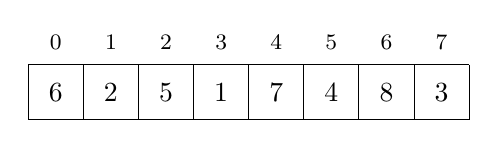
\begin{tikzpicture}[scale=0.7]
\draw (0,0) grid (8,1);
\node at (0.5,0.5) {$6$};
\node at (1.5,0.5) {$2$};
\node at (2.5,0.5) {$5$};
\node at (3.5,0.5) {$1$};
\node at (4.5,0.5) {$7$};
\node at (5.5,0.5) {$4$};
\node at (6.5,0.5) {$8$};
\node at (7.5,0.5) {$3$};

\footnotesize
\node at (0.5,1.4) {$0$};
\node at (1.5,1.4) {$1$};
\node at (2.5,1.4) {$2$};
\node at (3.5,1.4) {$3$};
\node at (4.5,1.4) {$4$};
\node at (5.5,1.4) {$5$};
\node at (6.5,1.4) {$6$};
\node at (7.5,1.4) {$7$};
\end{tikzpicture}
\end{center}
中，最长递增子序列包含 4 个元素：
\begin{center}
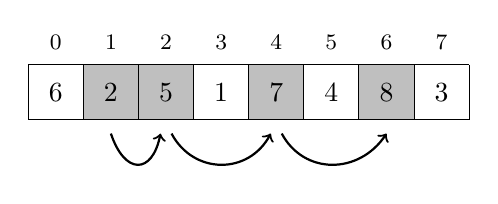
\begin{tikzpicture}[scale=0.7]
\fill[color=lightgray] (1,0) rectangle (2,1);
\fill[color=lightgray] (2,0) rectangle (3,1);
\fill[color=lightgray] (4,0) rectangle (5,1);
\fill[color=lightgray] (6,0) rectangle (7,1);
\draw (0,0) grid (8,1);
\node at (0.5,0.5) {$6$};
\node at (1.5,0.5) {$2$};
\node at (2.5,0.5) {$5$};
\node at (3.5,0.5) {$1$};
\node at (4.5,0.5) {$7$};
\node at (5.5,0.5) {$4$};
\node at (6.5,0.5) {$8$};
\node at (7.5,0.5) {$3$};

\draw[thick,->] (1.5,-0.25) .. controls (1.75,-1.00) and (2.25,-1.00) .. (2.4,-0.25);
\draw[thick,->] (2.6,-0.25) .. controls (3.0,-1.00) and (4.0,-1.00) .. (4.4,-0.25);
\draw[thick,->] (4.6,-0.25) .. controls (5.0,-1.00) and (6.0,-1.00) .. (6.5,-0.25);

\footnotesize
\node at (0.5,1.4) {$0$};
\node at (1.5,1.4) {$1$};
\node at (2.5,1.4) {$2$};
\node at (3.5,1.4) {$3$};
\node at (4.5,1.4) {$4$};
\node at (5.5,1.4) {$5$};
\node at (6.5,1.4) {$6$};
\node at (7.5,1.4) {$7$};
\end{tikzpicture}
\end{center}

令 $\texttt{length}(k)$ 表示以位置 $k$ 结尾的最长递增子序列长度。因此，计算出所有 $0\le k\le n-1$ 的 $\texttt{length}(k)$，就能得到最长递增子序列的长度。对于上述数组，函数值如下：
\[
\begin{array}{lcl}
\texttt{length}(0) & = & 1 \\
\texttt{length}(1) & = & 1 \\
\texttt{length}(2) & = & 2 \\
\texttt{length}(3) & = & 1 \\
\texttt{length}(4) & = & 3 \\
\texttt{length}(5) & = & 2 \\
\texttt{length}(6) & = & 4 \\
\texttt{length}(7) & = & 2 \\
\end{array}
\]

例如，$\texttt{length}(6)=4$，因为以位置 6 结尾的最长递增子序列含有 4 个元素。

为计算 $\texttt{length}(k)$，应找到位置 $i<k$，使 $\texttt{array}[i]<\texttt{array}[k]$ 且 $\texttt{length}(i)$ 尽可能大。于是 $\texttt{length}(k)=\texttt{length}(i)+1$，因为这是把 $\texttt{array}[k]$ 加入子序列的最优方式。若不存在这样的位置 $i$，则 $\texttt{length}(k)=1$，即子序列只含 $\texttt{array}[k]$。

由于所有函数值都能由较小的函数值计算，可以使用动态规划。下列代码将函数值存入数组 $\texttt{length}$。

\begin{lstlisting}
for (int k = 0; k < n; k++) {
    length[k] = 1;
    for (int i = 0; i < k; i++) {
        if (array[i] < array[k]) {
            length[k] = max(length[k],length[i]+1);
        }
    }
}
\end{lstlisting}

该代码包含两层嵌套循环，时间复杂度为 $O(n^2)$。不过，也可以在 $O(n\log n)$ 时间内更高效地完成这一动态规划计算。你能找到方法吗？

\section{网格中的路径}

下一个问题是在 $n\times n$ 网格中寻找一条从左上角到右下角、只能向下或向右移动的路径。每个方格包含一个正整数，需要让路径上数值之和尽可能大。

下图展示了网格中的一条最优路径：
\begin{center}
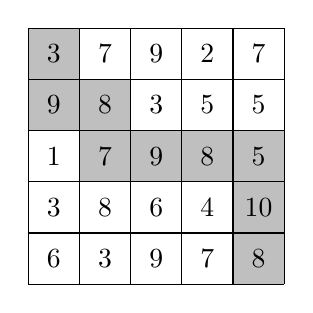
\begin{tikzpicture}[scale=.65]
  \begin{scope}
    \fill [color=lightgray] (0, 9) rectangle (1, 8);
    \fill [color=lightgray] (0, 8) rectangle (1, 7);
    \fill [color=lightgray] (1, 8) rectangle (2, 7);
    \fill [color=lightgray] (1, 7) rectangle (2, 6);
    \fill [color=lightgray] (2, 7) rectangle (3, 6);
    \fill [color=lightgray] (3, 7) rectangle (4, 6);
    \fill [color=lightgray] (4, 7) rectangle (5, 6);
    \fill [color=lightgray] (4, 6) rectangle (5, 5);
    \fill [color=lightgray] (4, 5) rectangle (5, 4);
    \draw (0, 4) grid (5, 9);
    \node at (0.5,8.5) {3};
    \node at (1.5,8.5) {7};
    \node at (2.5,8.5) {9};
    \node at (3.5,8.5) {2};
    \node at (4.5,8.5) {7};
    \node at (0.5,7.5) {9};
    \node at (1.5,7.5) {8};
    \node at (2.5,7.5) {3};
    \node at (3.5,7.5) {5};
    \node at (4.5,7.5) {5};
    \node at (0.5,6.5) {1};
    \node at (1.5,6.5) {7};
    \node at (2.5,6.5) {9};
    \node at (3.5,6.5) {8};
    \node at (4.5,6.5) {5};
    \node at (0.5,5.5) {3};
    \node at (1.5,5.5) {8};
    \node at (2.5,5.5) {6};
    \node at (3.5,5.5) {4};
    \node at (4.5,5.5) {10};
    \node at (0.5,4.5) {6};
    \node at (1.5,4.5) {3};
    \node at (2.5,4.5) {9};
    \node at (3.5,4.5) {7};
    \node at (4.5,4.5) {8};
  \end{scope}
\end{tikzpicture}
\end{center}
路径上的数值之和为 67，这是从左上角到右下角的路径所能取得的最大和。

假设网格行列均从 1 编号到 $n$，$\texttt{value}[y][x]$ 等于方格 $(y,x)$ 中的值。令 $\texttt{sum}(y,x)$ 表示从左上角到方格 $(y,x)$ 的路径最大和，则 $\texttt{sum}(n,n)$ 就是从左上角到右下角的最大和。例如，在上述网格中，$\texttt{sum}(5,5)=67$。

可以按如下递推式计算这些和：
\[ \texttt{sum}(y,x) = \max(\texttt{sum}(y,x-1),\texttt{sum}(y-1,x))+\texttt{value}[y][x]\]


该递推式基于如下观察：以方格 $(y,x)$ 结尾的路径只能来自方格 $(y,x-1)$ 或 $(y-1,x)$：
\begin{center}
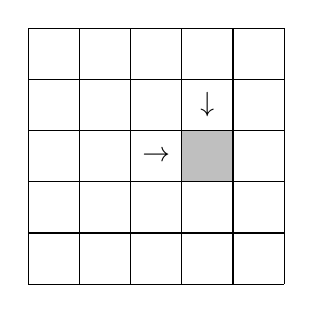
\begin{tikzpicture}[scale=.65]
  \begin{scope}
    \fill [color=lightgray] (3, 7) rectangle (4, 6);
    \draw (0, 4) grid (5, 9);
    
    \node at (2.5,6.5) {$\rightarrow$};
    \node at (3.5,7.5) {$\downarrow$};
    
  \end{scope}
\end{tikzpicture}
\end{center}

因此，应选择使总和最大的方向。规定当 $y=0$ 或 $x=0$ 时 $\texttt{sum}(y,x)=0$（因为不存在这样的路径），这样递推式在 $y=1$ 或 $x=1$ 时也适用。

由于函数 \texttt{sum} 有两个参数，动态规划数组也有两个维度。例如，可以使用数组
\begin{lstlisting}
int sum[N][N];
\end{lstlisting}
并按如下方式计算：
\begin{lstlisting}
for (int y = 1; y <= n; y++) {
    for (int x = 1; x <= n; x++) {
        sum[y][x] = max(sum[y][x-1],sum[y-1][x])+value[y][x];
    }
}
\end{lstlisting}
算法的时间复杂度为 $O(n^2)$。

\section{背包问题}

\index{knapsack}

\key{背包问题}是指给定一组物品，要求找出具有某些性质的子集的一类问题。背包问题通常可以用动态规划解决。

本节重点讨论如下问题：给定重量列表 $[w_1,w_2,\ldots,w_n]$，确定用这些重量能够组成的所有总和。例如，当重量为 $[1,3,3,5]$ 时，可以组成下列总和：

\begin{center}
\begin{tabular}{rrrrrrrrrrrrr}
 0 & 1 & 2 & 3 & 4 & 5 & 6 & 7 & 8 & 9 & 10 & 11 & 12 \\
\hline
 X & X & & X & X & X & X & X & X & X & & X & X \\
\end{tabular}
\end{center}

此时，$0\ldots 12$ 之间除 2 和 10 外的所有总和都可以组成。例如，选择重量 $[1,3,3]$ 即可组成总和 7。

为解决该问题，考虑只使用前 $k$ 个重量来组成总和的子问题。如果能用前 $k$ 个重量组成总和 $x$，令 $\texttt{possible}(x,k)=\textrm{true}$，否则令其为 $\textrm{false}$。函数值可按如下方式递推：
\[ \texttt{possible}(x,k) = \texttt{possible}(x-w_k,k-1) \lor \texttt{possible}(x,k-1) \]
这个公式基于这样一个事实：组成总和时可以选择使用或不使用重量 $w_k$。若使用 $w_k$，剩余任务是用前 $k-1$ 个重量组成 $x-w_k$；若不使用 $w_k$，则要用前 $k-1$ 个重量组成 $x$。基本情形为
\begin{equation*}
    \texttt{possible}(x,0) = \begin{cases}
               \textrm{true}    & x = 0\\
               \textrm{false}   & x \neq 0 \\
           \end{cases}
\end{equation*}
因为不使用任何重量时只能组成总和 0。

下表给出了重量 $[1,3,3,5]$ 对应的所有函数值（符号“X”表示值为真）：

\begin{center}
\begin{tabular}{r|rrrrrrrrrrrrr}
$k \backslash x$ & 0 & 1 & 2 & 3 & 4 & 5 & 6 & 7 & 8 & 9 & 10 & 11 & 12 \\
\hline
 0 & X & \\
 1 & X & X \\
 2 & X & X & & X & X \\
 3 & X & X & & X & X & & X & X \\
 4 & X & X & & X & X & X & X & X & X & X & & X & X \\
\end{tabular}
\end{center}

计算这些值后，$\texttt{possible}(x,n)$ 表示能否使用\emph{全部}重量中的若干个组成总和 $x$。

令 $W$ 表示所有重量之和。下列时间复杂度为 $O(nW)$ 的动态规划解法与递归函数相对应：
\begin{lstlisting}
possible[0][0] = true;
for (int k = 1; k <= n; k++) {
    for (int x = 0; x <= W; x++) {
        if (x-w[k] >= 0) possible[x][k] |= possible[x-w[k]][k-1];
        possible[x][k] |= possible[x][k-1];
    }
}
\end{lstlisting}

不过，还有一种更好的实现，只使用一维数组 $\texttt{possible}[x]$ 表示能否构造出总和为 $x$ 的子集。技巧是对每个新重量从右向左更新数组：
\begin{lstlisting}
possible[0] = true;
for (int k = 1; k <= n; k++) {
    for (int x = W; x >= 0; x--) {
        if (possible[x]) possible[x+w[k]] = true;
    }
}
\end{lstlisting}

这里的一般思想可用于许多背包问题。例如，若给定带有重量和价值的物品，可以对每个重量总和求出子集的最大价值总和。

\section{编辑距离}

\index{edit distance}
\index{Levenshtein distance}

\key{编辑距离}，也称\key{Levenshtein 距离}\footnote{该距离以 V. I. Levenshtein 命名，他在研究二进制编码时研究了这一距离 \cite{lev66}。}，是将一个字符串变为另一个字符串所需的最少编辑操作数。允许的编辑操作如下：
\begin{itemize}
\item 插入一个字符（例如 \texttt{ABC} $\rightarrow$ \texttt{ABCA}）
\item 删除一个字符（例如 \texttt{ABC} $\rightarrow$ \texttt{AC}）
\item 修改一个字符（例如 \texttt{ABC} $\rightarrow$ \texttt{ADC}）
\end{itemize}

例如，\texttt{LOVE} 与 \texttt{MOVIE} 之间的编辑距离为 2，因为可以先执行 \texttt{LOVE} $\rightarrow$ \texttt{MOVE}（修改），再执行 \texttt{MOVE} $\rightarrow$ \texttt{MOVIE}（插入）。这是最少操作数，因为显然一次操作不足以完成转换。

设给定长度为 $n$ 的字符串 \texttt{x} 和长度为 $m$ 的字符串 \texttt{y}，要计算二者的编辑距离。定义函数 $\texttt{distance}(a,b)$ 表示前缀 $\texttt{x}[0\ldots a]$ 与 $\texttt{y}[0\ldots b]$ 之间的编辑距离，则 \texttt{x} 和 \texttt{y} 的编辑距离为 $\texttt{distance}(n-1,m-1)$。

可以按如下方式计算 \texttt{distance}：
\begin{equation*}
\begin{split}
\texttt{distance}(a,b) = \min(& \texttt{distance}(a,b-1)+1, \\
                           & \texttt{distance}(a-1,b)+1, \\
                           & \texttt{distance}(a-1,b-1)+\texttt{cost}(a,b)).
\end{split}
\end{equation*}
当 $\texttt{x}[a]=\texttt{y}[b]$ 时，$\texttt{cost}(a,b)=0$，否则 $\texttt{cost}(a,b)=1$。该公式考虑了如下编辑字符串 \texttt{x} 的方式：
\begin{itemize}
\item $\texttt{distance}(a,b-1)$：在 \texttt{x} 末尾插入一个字符
\item $\texttt{distance}(a-1,b)$：删除 \texttt{x} 的最后一个字符
\item $\texttt{distance}(a-1,b-1)$：匹配或修改 \texttt{x} 的最后一个字符
\end{itemize}
前两种情形需要一次编辑操作（插入或删除）。在最后一种情形中，若 $\texttt{x}[a]=\texttt{y}[b]$，无需编辑即可匹配最后一个字符；否则需要一次修改操作。

下表给出了示例中的 \texttt{distance} 值：
\begin{center}
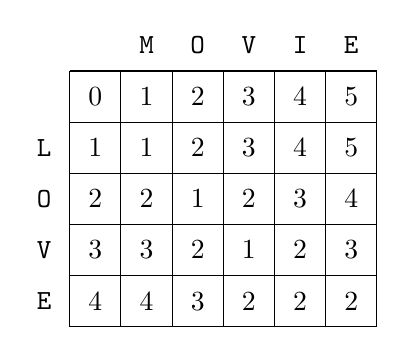
\begin{tikzpicture}[scale=.65]
  \begin{scope}
    %\fill [color=lightgray] (5, -3) rectangle (6, -4);
    \draw (1, -1) grid (7, -6);
    
    \node at (0.5,-2.5) {\texttt{L}};
    \node at (0.5,-3.5) {\texttt{O}};
    \node at (0.5,-4.5) {\texttt{V}};
    \node at (0.5,-5.5) {\texttt{E}};

    \node at (2.5,-0.5) {\texttt{M}};
    \node at (3.5,-0.5) {\texttt{O}};
    \node at (4.5,-0.5) {\texttt{V}};
    \node at (5.5,-0.5) {\texttt{I}};
    \node at (6.5,-0.5) {\texttt{E}};

    \node at (1.5,-1.5) {$0$};
    \node at (1.5,-2.5) {$1$};
    \node at (1.5,-3.5) {$2$};
    \node at (1.5,-4.5) {$3$};
    \node at (1.5,-5.5) {$4$};
    \node at (2.5,-1.5) {$1$};
    \node at (2.5,-2.5) {$1$};
    \node at (2.5,-3.5) {$2$};
    \node at (2.5,-4.5) {$3$};
    \node at (2.5,-5.5) {$4$};
    \node at (3.5,-1.5) {$2$};
    \node at (3.5,-2.5) {$2$};
    \node at (3.5,-3.5) {$1$};
    \node at (3.5,-4.5) {$2$};
    \node at (3.5,-5.5) {$3$};
    \node at (4.5,-1.5) {$3$};
    \node at (4.5,-2.5) {$3$};
    \node at (4.5,-3.5) {$2$};
    \node at (4.5,-4.5) {$1$};
    \node at (4.5,-5.5) {$2$};
    \node at (5.5,-1.5) {$4$};
    \node at (5.5,-2.5) {$4$};
    \node at (5.5,-3.5) {$3$};
    \node at (5.5,-4.5) {$2$};
    \node at (5.5,-5.5) {$2$};
    \node at (6.5,-1.5) {$5$};
    \node at (6.5,-2.5) {$5$};
    \node at (6.5,-3.5) {$4$};
    \node at (6.5,-4.5) {$3$};
    \node at (6.5,-5.5) {$2$};
  \end{scope}
\end{tikzpicture}
\end{center}

表格右下角表明 \texttt{LOVE} 与 \texttt{MOVIE} 的编辑距离为 2。该表还展示了如何构造最短编辑操作序列。此时路径如下：

\begin{center}
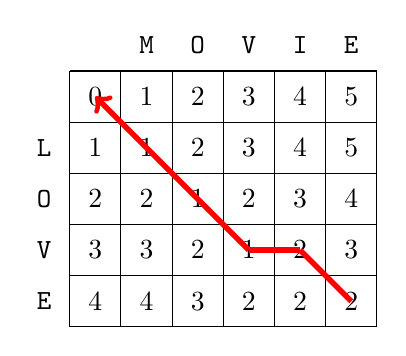
\begin{tikzpicture}[scale=.65]
  \begin{scope}
    \draw (1, -1) grid (7, -6);
    
    \node at (0.5,-2.5) {\texttt{L}};
    \node at (0.5,-3.5) {\texttt{O}};
    \node at (0.5,-4.5) {\texttt{V}};
    \node at (0.5,-5.5) {\texttt{E}};

    \node at (2.5,-0.5) {\texttt{M}};
    \node at (3.5,-0.5) {\texttt{O}};
    \node at (4.5,-0.5) {\texttt{V}};
    \node at (5.5,-0.5) {\texttt{I}};
    \node at (6.5,-0.5) {\texttt{E}};

    \node at (1.5,-1.5) {$0$};
    \node at (1.5,-2.5) {$1$};
    \node at (1.5,-3.5) {$2$};
    \node at (1.5,-4.5) {$3$};
    \node at (1.5,-5.5) {$4$};
    \node at (2.5,-1.5) {$1$};
    \node at (2.5,-2.5) {$1$};
    \node at (2.5,-3.5) {$2$};
    \node at (2.5,-4.5) {$3$};
    \node at (2.5,-5.5) {$4$};
    \node at (3.5,-1.5) {$2$};
    \node at (3.5,-2.5) {$2$};
    \node at (3.5,-3.5) {$1$};
    \node at (3.5,-4.5) {$2$};
    \node at (3.5,-5.5) {$3$};
    \node at (4.5,-1.5) {$3$};
    \node at (4.5,-2.5) {$3$};
    \node at (4.5,-3.5) {$2$};
    \node at (4.5,-4.5) {$1$};
    \node at (4.5,-5.5) {$2$};
    \node at (5.5,-1.5) {$4$};
    \node at (5.5,-2.5) {$4$};
    \node at (5.5,-3.5) {$3$};
    \node at (5.5,-4.5) {$2$};
    \node at (5.5,-5.5) {$2$};
    \node at (6.5,-1.5) {$5$};
    \node at (6.5,-2.5) {$5$};
    \node at (6.5,-3.5) {$4$};
    \node at (6.5,-4.5) {$3$};
    \node at (6.5,-5.5) {$2$};

    \path[draw=red,thick,-,line width=2pt] (6.5,-5.5) -- (5.5,-4.5);
    \path[draw=red,thick,-,line width=2pt] (5.5,-4.5) -- (4.5,-4.5);
    \path[draw=red,thick,->,line width=2pt] (4.5,-4.5) -- (1.5,-1.5);
  \end{scope}
\end{tikzpicture}
\end{center}

\texttt{LOVE} 与 \texttt{MOVIE} 的最后一个字符相同，所以二者的编辑距离等于 \texttt{LOV} 与 \texttt{MOVI} 的编辑距离。可以用一次编辑操作从 \texttt{MOVI} 中删除字符 \texttt{I}，因此该距离比 \texttt{LOV} 与 \texttt{MOV} 的编辑距离大一，依此类推。

\section{铺砖方案计数}

有时，动态规划状态会比固定的数字组合更加复杂。例如，考虑用 $1\times 2$ 和 $2\times 1$ 的砖铺满 $n\times m$ 网格的不同方案数。下面是 $4\times 7$ 网格的一种合法方案：
\begin{center}
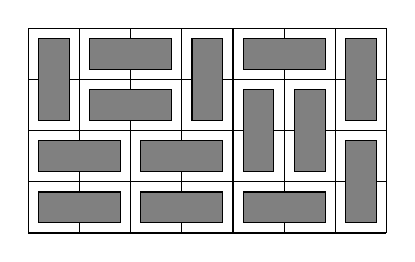
\begin{tikzpicture}[scale=.65]
    \draw (0,0) grid (7,4);
    \draw[fill=gray] (0+0.2,0+0.2) rectangle (2-0.2,1-0.2);
    \draw[fill=gray] (2+0.2,0+0.2) rectangle (4-0.2,1-0.2);
    \draw[fill=gray] (4+0.2,0+0.2) rectangle (6-0.2,1-0.2);
    \draw[fill=gray] (0+0.2,1+0.2) rectangle (2-0.2,2-0.2);
    \draw[fill=gray] (2+0.2,1+0.2) rectangle (4-0.2,2-0.2);
    \draw[fill=gray] (1+0.2,2+0.2) rectangle (3-0.2,3-0.2);
    \draw[fill=gray] (1+0.2,3+0.2) rectangle (3-0.2,4-0.2);
    \draw[fill=gray] (4+0.2,3+0.2) rectangle (6-0.2,4-0.2);

    \draw[fill=gray] (0+0.2,2+0.2) rectangle (1-0.2,4-0.2);
    \draw[fill=gray] (3+0.2,2+0.2) rectangle (4-0.2,4-0.2);
    \draw[fill=gray] (6+0.2,2+0.2) rectangle (7-0.2,4-0.2);
    \draw[fill=gray] (4+0.2,1+0.2) rectangle (5-0.2,3-0.2);
    \draw[fill=gray] (5+0.2,1+0.2) rectangle (6-0.2,3-0.2);
    \draw[fill=gray] (6+0.2,0+0.2) rectangle (7-0.2,2-0.2);

\end{tikzpicture}
\end{center}
而方案总数为 781。

可以逐行遍历网格，用动态规划解决该问题。解中的每一行都可以表示为一个长度为 $m$ 的字符串，字符取自集合 $\{\sqcap,\sqcup,\sqsubset,\sqsupset\}$。例如，上述解由四行组成，对应下列字符串：
\begin{itemize}
\item
$\sqcap \sqsubset \sqsupset \sqcap \sqsubset \sqsupset \sqcap$
\item
$\sqcup \sqsubset \sqsupset \sqcup \sqcap \sqcap \sqcup$
\item
$\sqsubset \sqsupset \sqsubset \sqsupset \sqcup \sqcup \sqcap$ 
\item
$\sqsubset \sqsupset \sqsubset \sqsupset \sqsubset \sqsupset \sqcup$
\end{itemize}

令 $\texttt{count}(k,x)$ 表示构造网格第 $1\ldots k$ 行，且第 $k$ 行对应字符串 $x$ 的方案数。这里可以使用动态规划，因为一行的状态只受前一行状态的约束。

一个解合法，当且仅当第 1 行不含字符 $\sqcup$，第 $n$ 行不含字符 $\sqcap$，并且所有相邻行都\emph{兼容}。例如，行
$\sqcup \sqsubset \sqsupset \sqcup \sqcap \sqcap \sqcup$ and
$\sqsubset \sqsupset \sqsubset \sqsupset \sqcup \sqcup \sqcap$ 
彼此兼容，而行
$\sqcap \sqsubset \sqsupset \sqcap \sqsubset \sqsupset \sqcap$ and
$\sqsubset \sqsupset \sqsubset \sqsupset \sqsubset \sqsupset \sqcup$
彼此不兼容。

由于每行含有 $m$ 个字符，每个字符有四种选择，不同行的数量至多为 $4^m$。因此，解法的时间复杂度为 $O(n4^{2m})$：每一行有 $O(4^m)$ 种可能状态，而对每种状态，前一行也有 $O(4^m)$ 种可能状态。实践中最好旋转网格，使较短边的长度为 $m$，因为因子 $4^{2m}$ 主导时间复杂度。

使用更紧凑的行表示可以提高效率。事实上，只需知道前一行的哪些列包含竖砖的上半部分。因此，可以只用字符 $\sqcap$ 和 $\Box$ 表示一行，其中 $\Box$ 综合表示字符 $\sqcup$、$\sqsubset$ 和 $\sqsupset$。采用这种表示后，只有 $2^m$ 种不同的行，时间复杂度为 $O(n2^{2m})$。

最后，还有一个令人惊讶的直接公式可以计算铺砖方案数\footnote{令人惊讶的是，该公式由两个彼此独立工作的研究团队于 1961 年发现 \cite{kas61,tem61}。}：
\[ \prod_{a=1}^{\lceil n/2 \rceil} \prod_{b=1}^{\lceil m/2 \rceil} 4 \cdot (\cos^2 \frac{\pi a}{n + 1} + \cos^2 \frac{\pi b}{m+1})\]
该公式非常高效，可以在 $O(nm)$ 时间内计算铺砖方案数。不过，由于答案是实数的乘积，使用该公式时的一个难题是如何精确保存中间结果。
